\chapter{Introducing MATSim}
\label{ch:introducing}
% ##################################################################################################################
\hfill \textbf{Author:} Andreas Horni 

\begin{center} 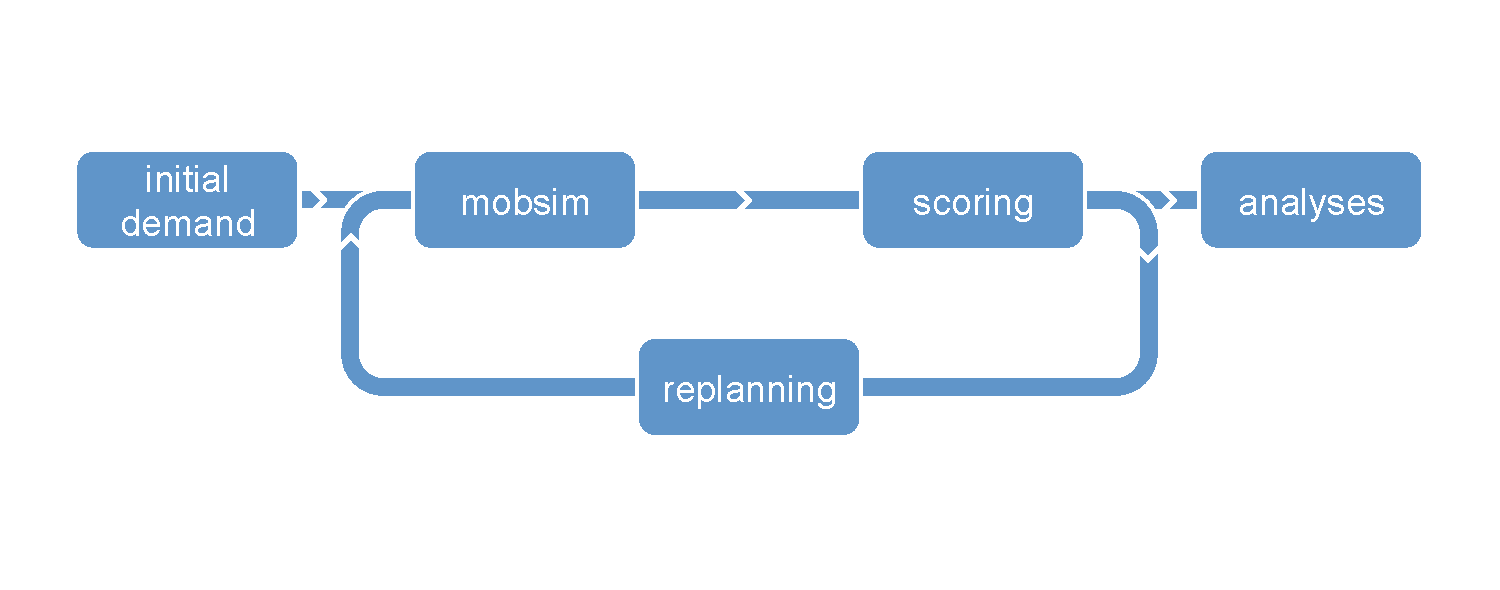
\includegraphics[width=0.7\textwidth, angle=0]{figures/matsimcycle.pdf} \end{center}

% ##################################################################################################################
A Glimpse at MATSim's History \who{Nagel, Axhausen}


MATSim Quickstart and Basics




The development of the multi-agent transport simulation MATSim \citep[][]{MATSIM-T_Webpage_2014, BalmerEtAl_TRR_2006} has started approximately a decade ago as a collaborative effort of Prof. Nagel (now: TU Berlin) and Prof. Axhausen (ETH Zurich). It has its roots in in \citet[][]{Axhausen_PhDThesis_1988} and in the transport simulation TRANSIMS \citep[][]{RaneyEtAl_LNCS_2002}, which was developed by Prof. Nagel as research team leader at the Los Alamos National Laboratory. As shown on the web page \citep[][]{MATSIM-T-Scenarios_Webpage_2013} and detailed in Chapter \ref{ch:scenariosprojects}, MATSim has been applied by local research groups world-wide for a dozen different regions.

MATSim is an activity-based, extendable, multi-agent simulation toolkit implemented in JAVA. It is open-source and can be downloaded freely at \citep[][]{MATSIM-T_Webpage_2014, SourceForge_Webpage_2014}. The framework is especially designed for large-scale scenarios, meaning that, the features of all models are generally stripped down to efficiently handle the base functionality, where emphasis has been also been laid on parallelization. For the network loading simulation, for example, a queue-based model is implemented, leaving out the very complex car-following behavior.

MATSim is based on a co-evolutionary principle (Section \ref{sec:co-ev}. While being in a competition for space-time slots on the transportation infrastructure with all the other agents, every agent iteratively optimizes its daily activity chain. This is done by running through the MATSim loop as depicted on the left in Figure \ref{fig:matsimcycle}. 

Every agent possesses a memory of a fixed number of day plans, where each plan is composed of a daily activity chain and an associated utility value (in MATSim called \emph{plan score}). For now, MATSim is conceptually designed to model a \emph{single day}, a common unit of analysis for activity-based models (see, for example, the review in \citet[][]{Bowman_TEC_2009_1}). In other words, basically, MATSim is a cross-sectional model. Nevertheless, in principle a longitudinal model could be implemented (Section \ref{sec:longitudinalscenario}).

In every iteration, prior to the simulation of the network loading \citep[e.g.,][]{Cetin_PhDThesis_2005} (\emph{execution}), every agent selects a plan from its memory. This selection is dependent on the plan utility. A certain share of the agents (often 10$\%$) is allowed to clone the selected plan and modify this clone (\emph{replanning}). For the method of successive averages (MSA) usually a decreasing share of travelers is reallocated to a new route to avoid oscillations. For MATSim, it has been shown that a variable replanning share can be productive as well and \emph{``increase overall performance of the system by a factor of three or more''} \citep[][p.7f]{CharyparEtAl_IATBR_2006}. For the network load microsimulation step multiple simulations are available and configurable \citep[][p.10f]{HorniEtAl_TechRep_IVT_2011_a}. 

Plan modification is implemented in the \emph{replanning} modules. Four choice dimensions are considered for now: time choice \citep[][]{BalmerEtAl_Timmermans_2005}, route choice \citep[]{LefebvreBalmer_STRC_2007}, mode choice, and destination choice. If an agent ends up with too many plans (configurable), the plan with the lowest score (configurable) is removed from the memory of this agent. The agents, which have not undergone replanning select between existing plans. The selection model is configurable; in many MATSim investigations, a model that generates a logit distribution for plan selection is used.

\ah{A:Tabelle mit Dimensions of Schedule angeben. Siehe MATSim-Pr�sentationen Prof. Axhausen.}

An iteration is completed by evaluating the agent's day described by the selected day plans (\emph{scoring}). The applied utility function is described below in Chapter \ref{ch:scoring}.

Starting from an initial demand, the iterative process is repeated until the average population score stabilizes, where the definition of the stopping criterion is subject of ongoing research initialized by \citet[][]{Meister_PhDThesis_2011, NagelFloetteroed_IATBR_2009}.

MATSim offers considerable customizability through its modular design approach. Although, replacing core modules, such as the network loading simulation is associated with a substantial effort \citep[][Section 2.4]{MATSim_Userguide_2014} in principle every module of the framework can be replaced. MATSim modules are detailed in Chapter \ref{ch:modules}.

% ------------
\createfigure%
{MATSim Cycle}%
{MATSim Cycle}%
{\label{fig:matsimcycle}}%
{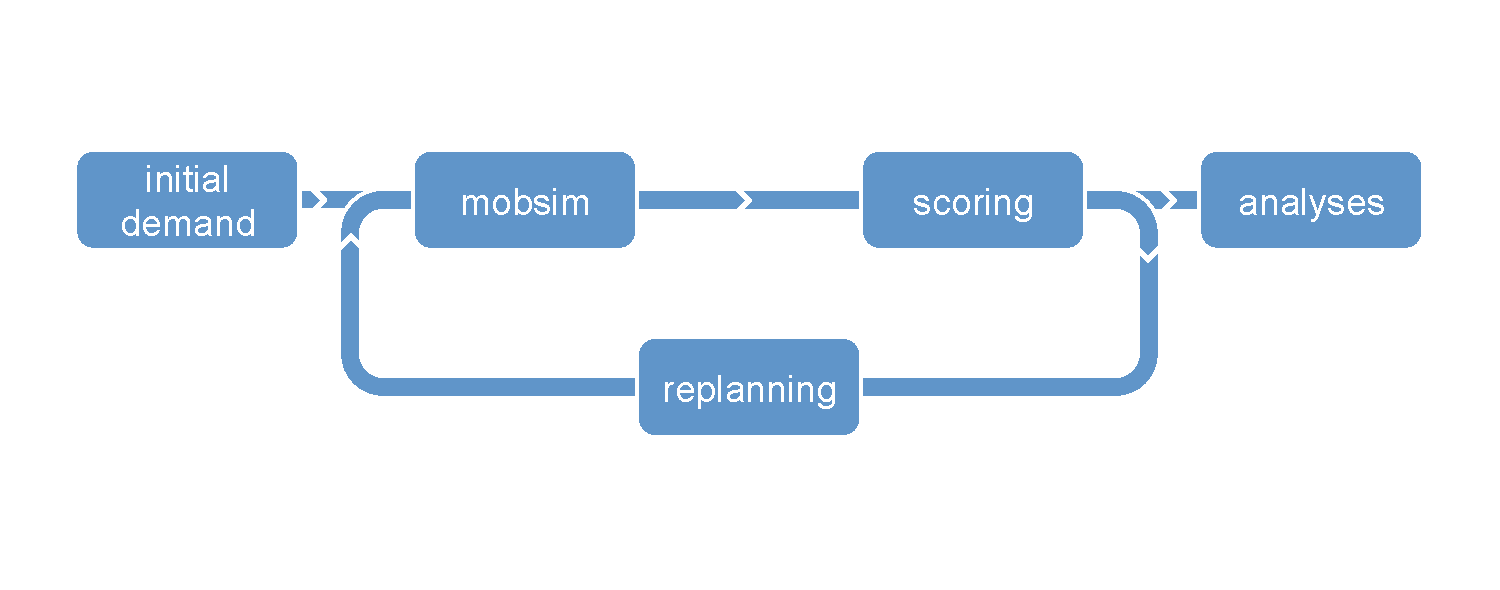
\includegraphics[width=0.99\textwidth, angle=0]{figures/matsimcycle.pdf}}%
{}

% ------------

\ah{link the text structurally more to the cycle, like in the user guide!} 

% ##################################################################################################################
\section{MATSim's Traffic Flow Model}
\label{sec:trafficflowmodel}
...


% ##################################################################################################################
\section{MATSim's Co-Evolutionary Algorithm}
\label{sec:co-ev}
As illustrated in Figure \ref{fig:ea}, the MATSim equilibrium is searched by a a \emph{\index{co-evolutionary algorithm}}. These algorithms co-evolve different species subject to interaction (e.g., competition). In MATSim, the individuals are represented by the plans of a person, where a person represents a species. By applying the co-evolutionary algorithm, optimization is performed in terms of agents' plans. Eventually, an equilibrium is reached subject to constraints, where the agents cannot further improve their plans unilaterally. When speaking in strict terms, there is a difference between application of an evolutionary algorithm and a \emph{co}-evolutionary algorithm. An evolutionary algorithm would lead to a system optimum as optimization is applied with a global (or population) fitness function. The co-evolutionary algorithm instead leads to a user equilibrium as optimization is performed in terms of \emph{individual} utility functions and within an agent's set of plans. At the moment, the MATSim co-evolutionary algorithm only includes mutation; recombination may come into play when joint day plans of family members, for example, are included in the future.

% ------------
\createfigure%
{Adopting a co-evolutionary algorithm in MATSim}%
{Adopting a co-evolutionary algorithm in MATSim}%
{\label{fig:ea}}%
{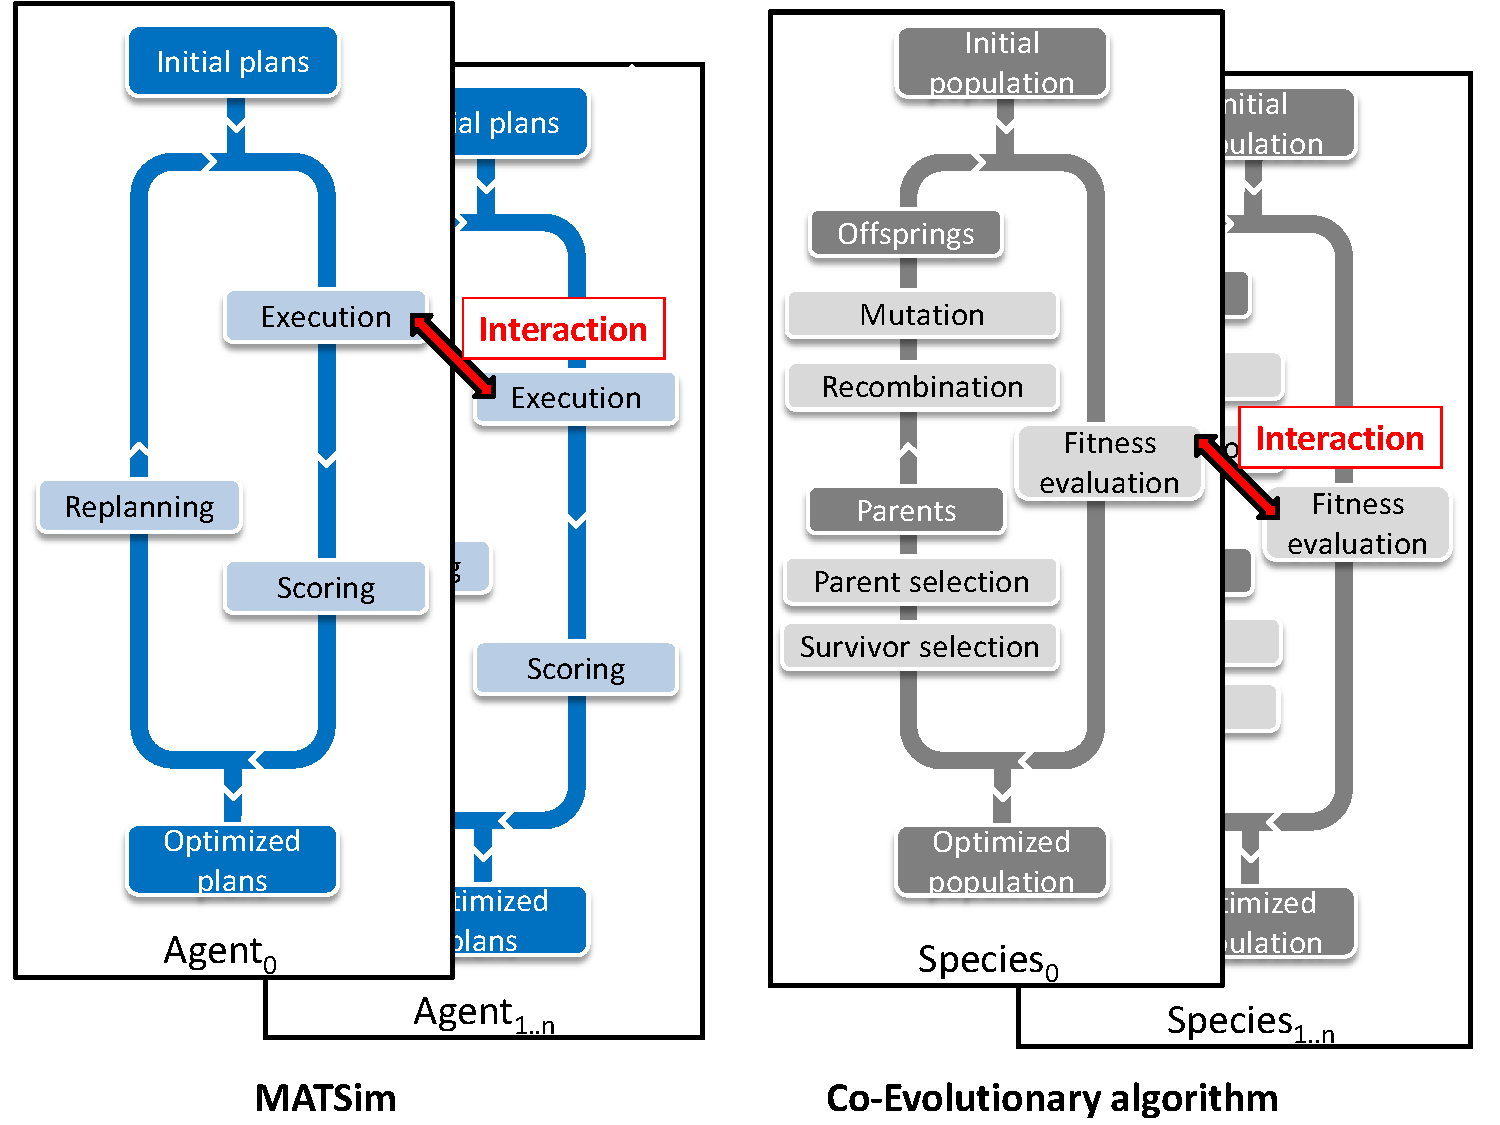
\includegraphics[width=0.99\textwidth, angle=0]{figures/MATSimVSea.pdf}}%
{}

% ------------

\ah{A little more co-ev theory. \\
Also practical knowledge \\
development of average score -> characteristic for co-ea \\
}

% ##################################################################################################################